\chapter{Scenario and Data Basis}
\label{sec:scenario}

The path planning framework developed in this work is evaluated in a representative
urban environment: the metropolitan area of Hamburg. This scenario provides a dense
network of potential vertiports connected via corridors and reflects the kinds of
challenges expected in future urban air mobility (UAM) operations.


\section{Vertiports}
Vertiports represent the take-off and landing sites for eVTOL aircraft. In this
study, a set of anonymized vertiport locations within Hamburg is used. Each
vertiport may contain one or more landing pads; for analysis, the average
latitude and longitude of all pads is taken as the node coordinate.
Figure~\ref{fig:vertiports_hamburg} illustrates the spatial distribution of
these vertiports across the city.

\begin{figure}[H]
    \centering
    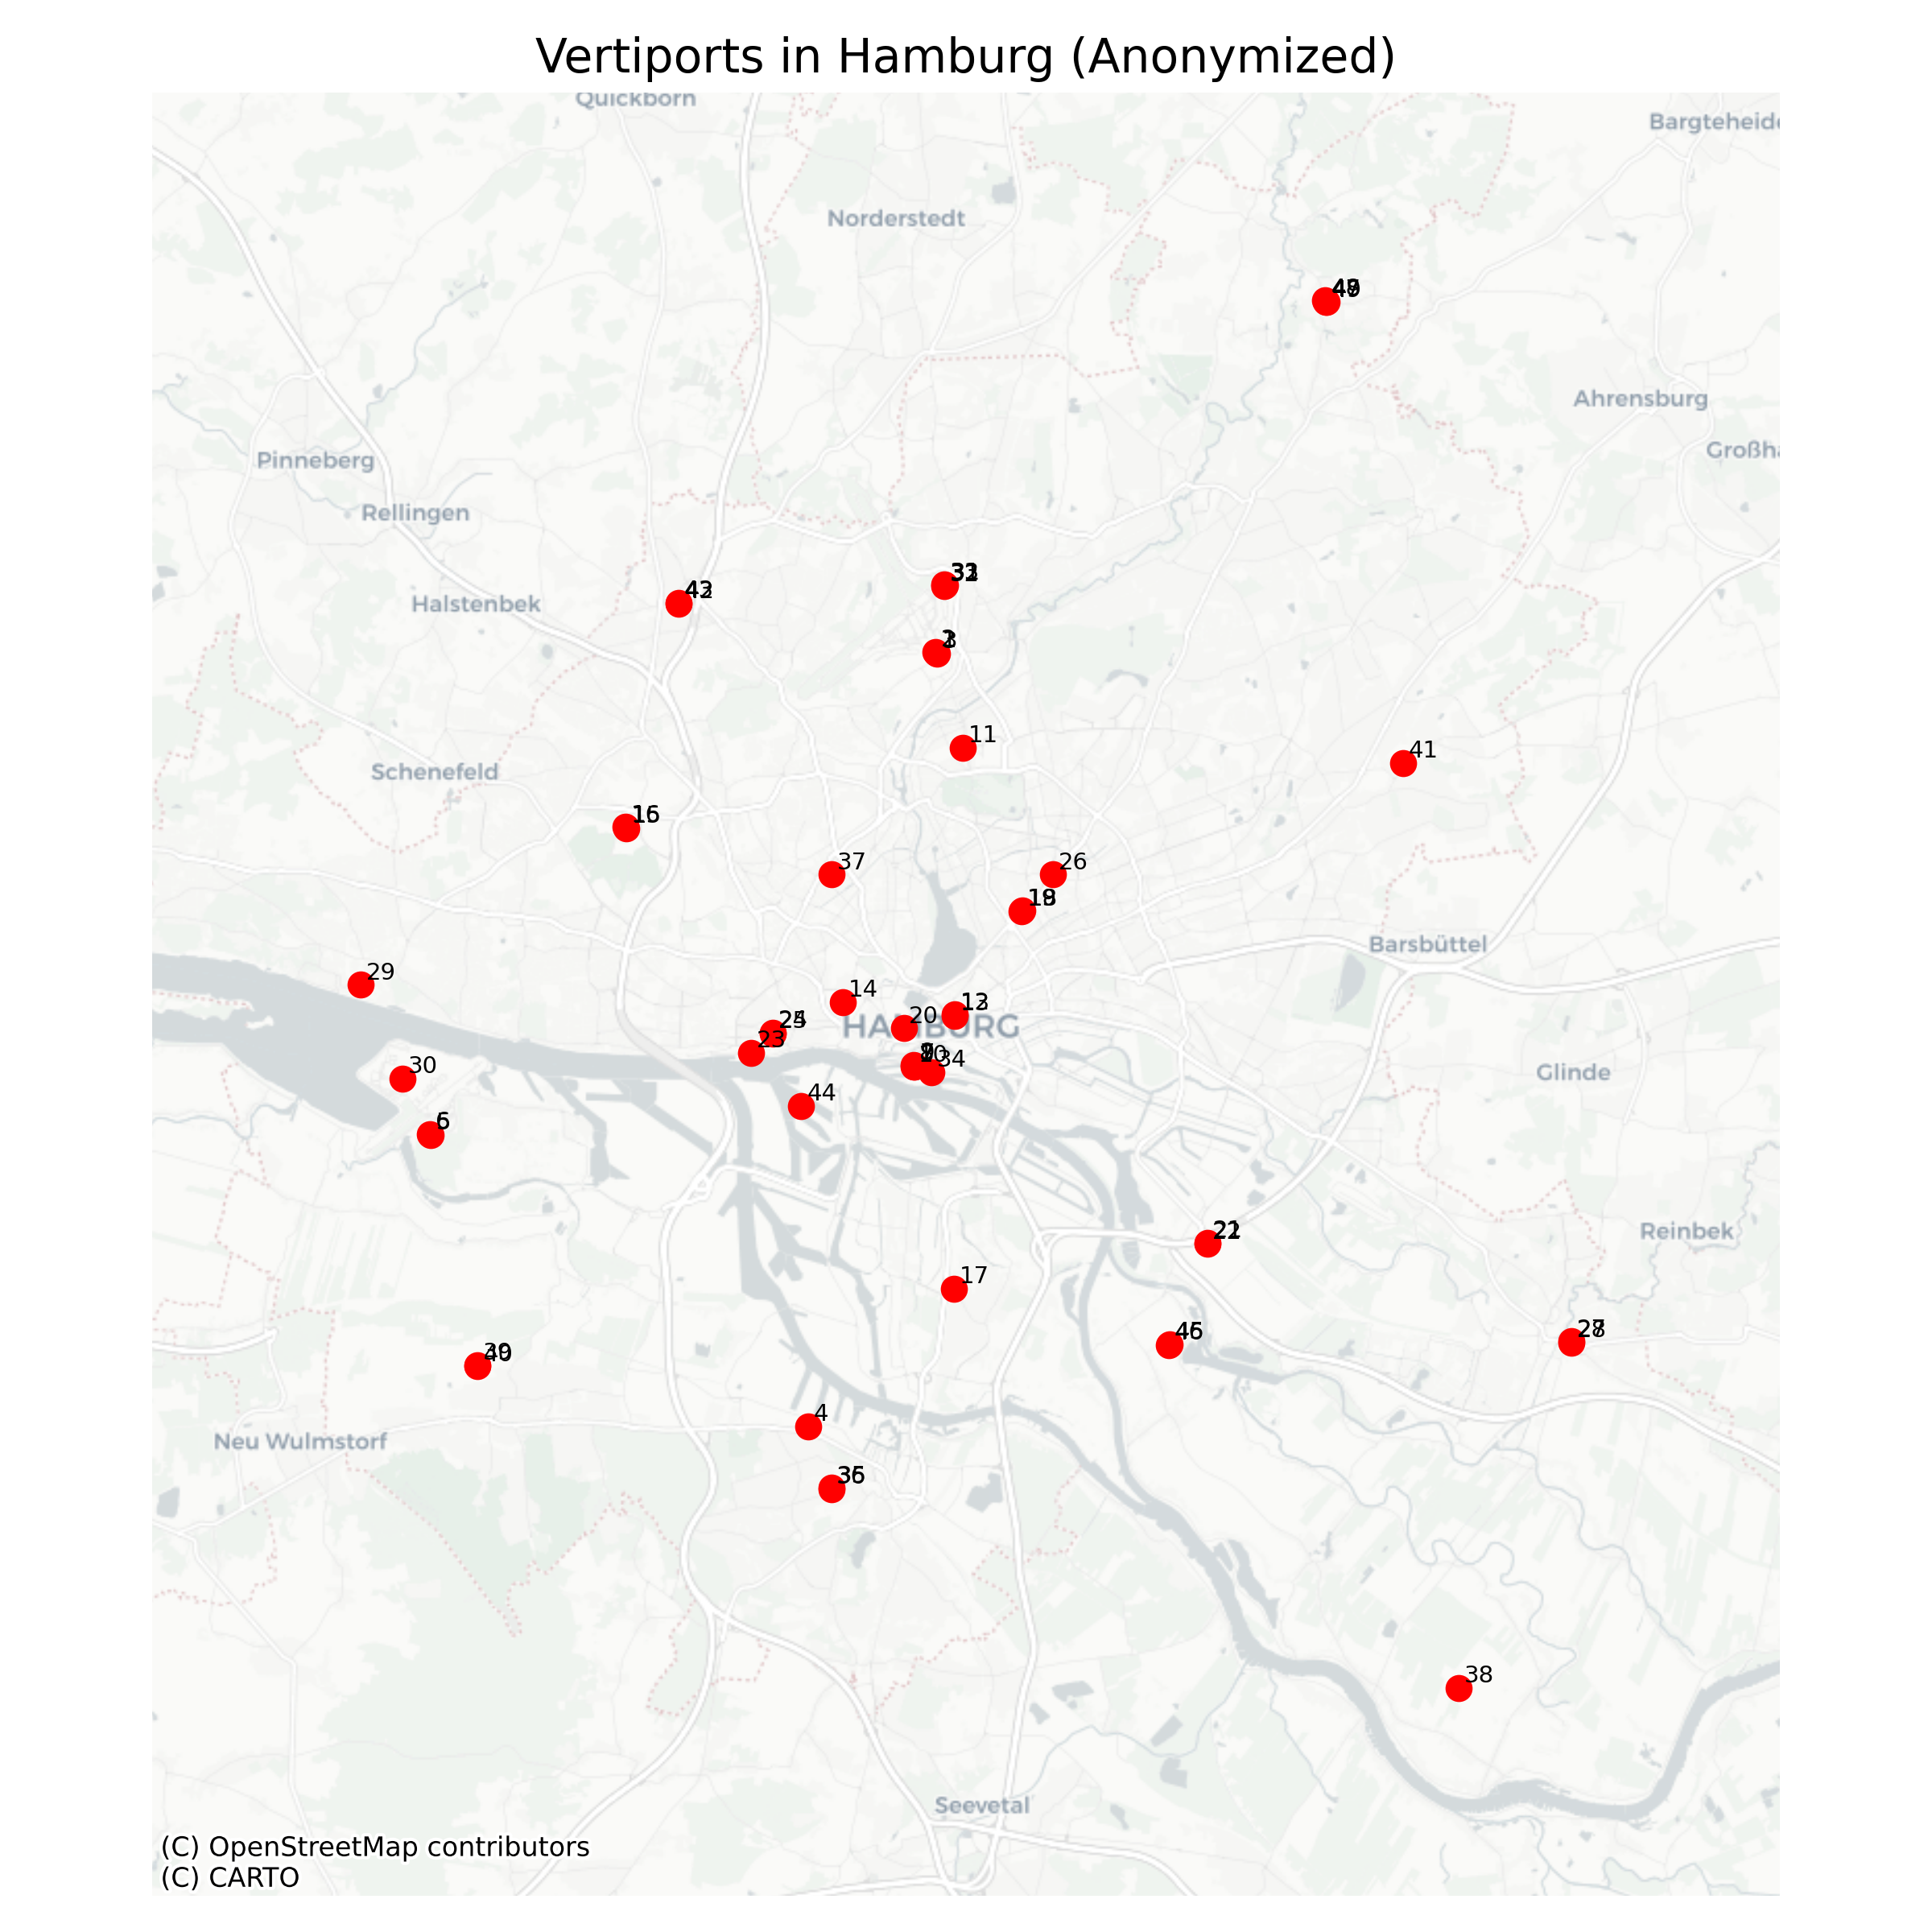
\includegraphics[width=0.8\textwidth]{figures/vertiports_hamburg.png}
    \caption{Vertiports in Hamburg (anonymized).}
    \label{fig:vertiports_hamburg}
\end{figure}

\subsection*{Corridors}
Corridors define the available airspace connections between vertiports and are
modeled as \emph{undirected} edges in the graph $G=(V,E)$. Geometrically, each
corridor is represented as a straight-line segment between two vertiports, and
the edge weight $d(u,v)$ corresponds to the geodesic (great-circle) distance
between their coordinates.

For the vertical structure, each corridor is placed at a fixed altitude layer.
According to the European Commission's U-space Blueprint \cite{eu_commission_2017},
a reference altitude of \SI{500}{ft} (approximately \SI{152}{m}) was adopted for
low-level airspace operations. In this work, a constant altitude of \SI{200}{m}
above ground level is used for the construction of corridors. Each corridor is
assigned a uniform width of \SI{20}{m}, representing a lateral safety buffer
around the nominal centerline.

For visualization and operator interaction, the corridor graph was also rendered in an interactive Cesium front-end (Fig. \ref{fig:corridors_comparison}, right). This allows the user to inspect the 3D geometry of the corridor network, vertical layering, and vertiport locations directly within a web-based interface.

Thus, the corridor model is characterized by the following specifications:
\begin{itemize}
    \item \textbf{Shape:} straight line between two vertiports;
    \item \textbf{Graph representation:} undirected edge with weight equal to geodesic distance;
    \item \textbf{Altitude:} constant \SI{200}{m} above ground level;
    \item \textbf{Width:} \SI{20}{m}.
\end{itemize}

\begin{figure}[H]
  \centering
  \begin{subfigure}{0.48\textwidth}
    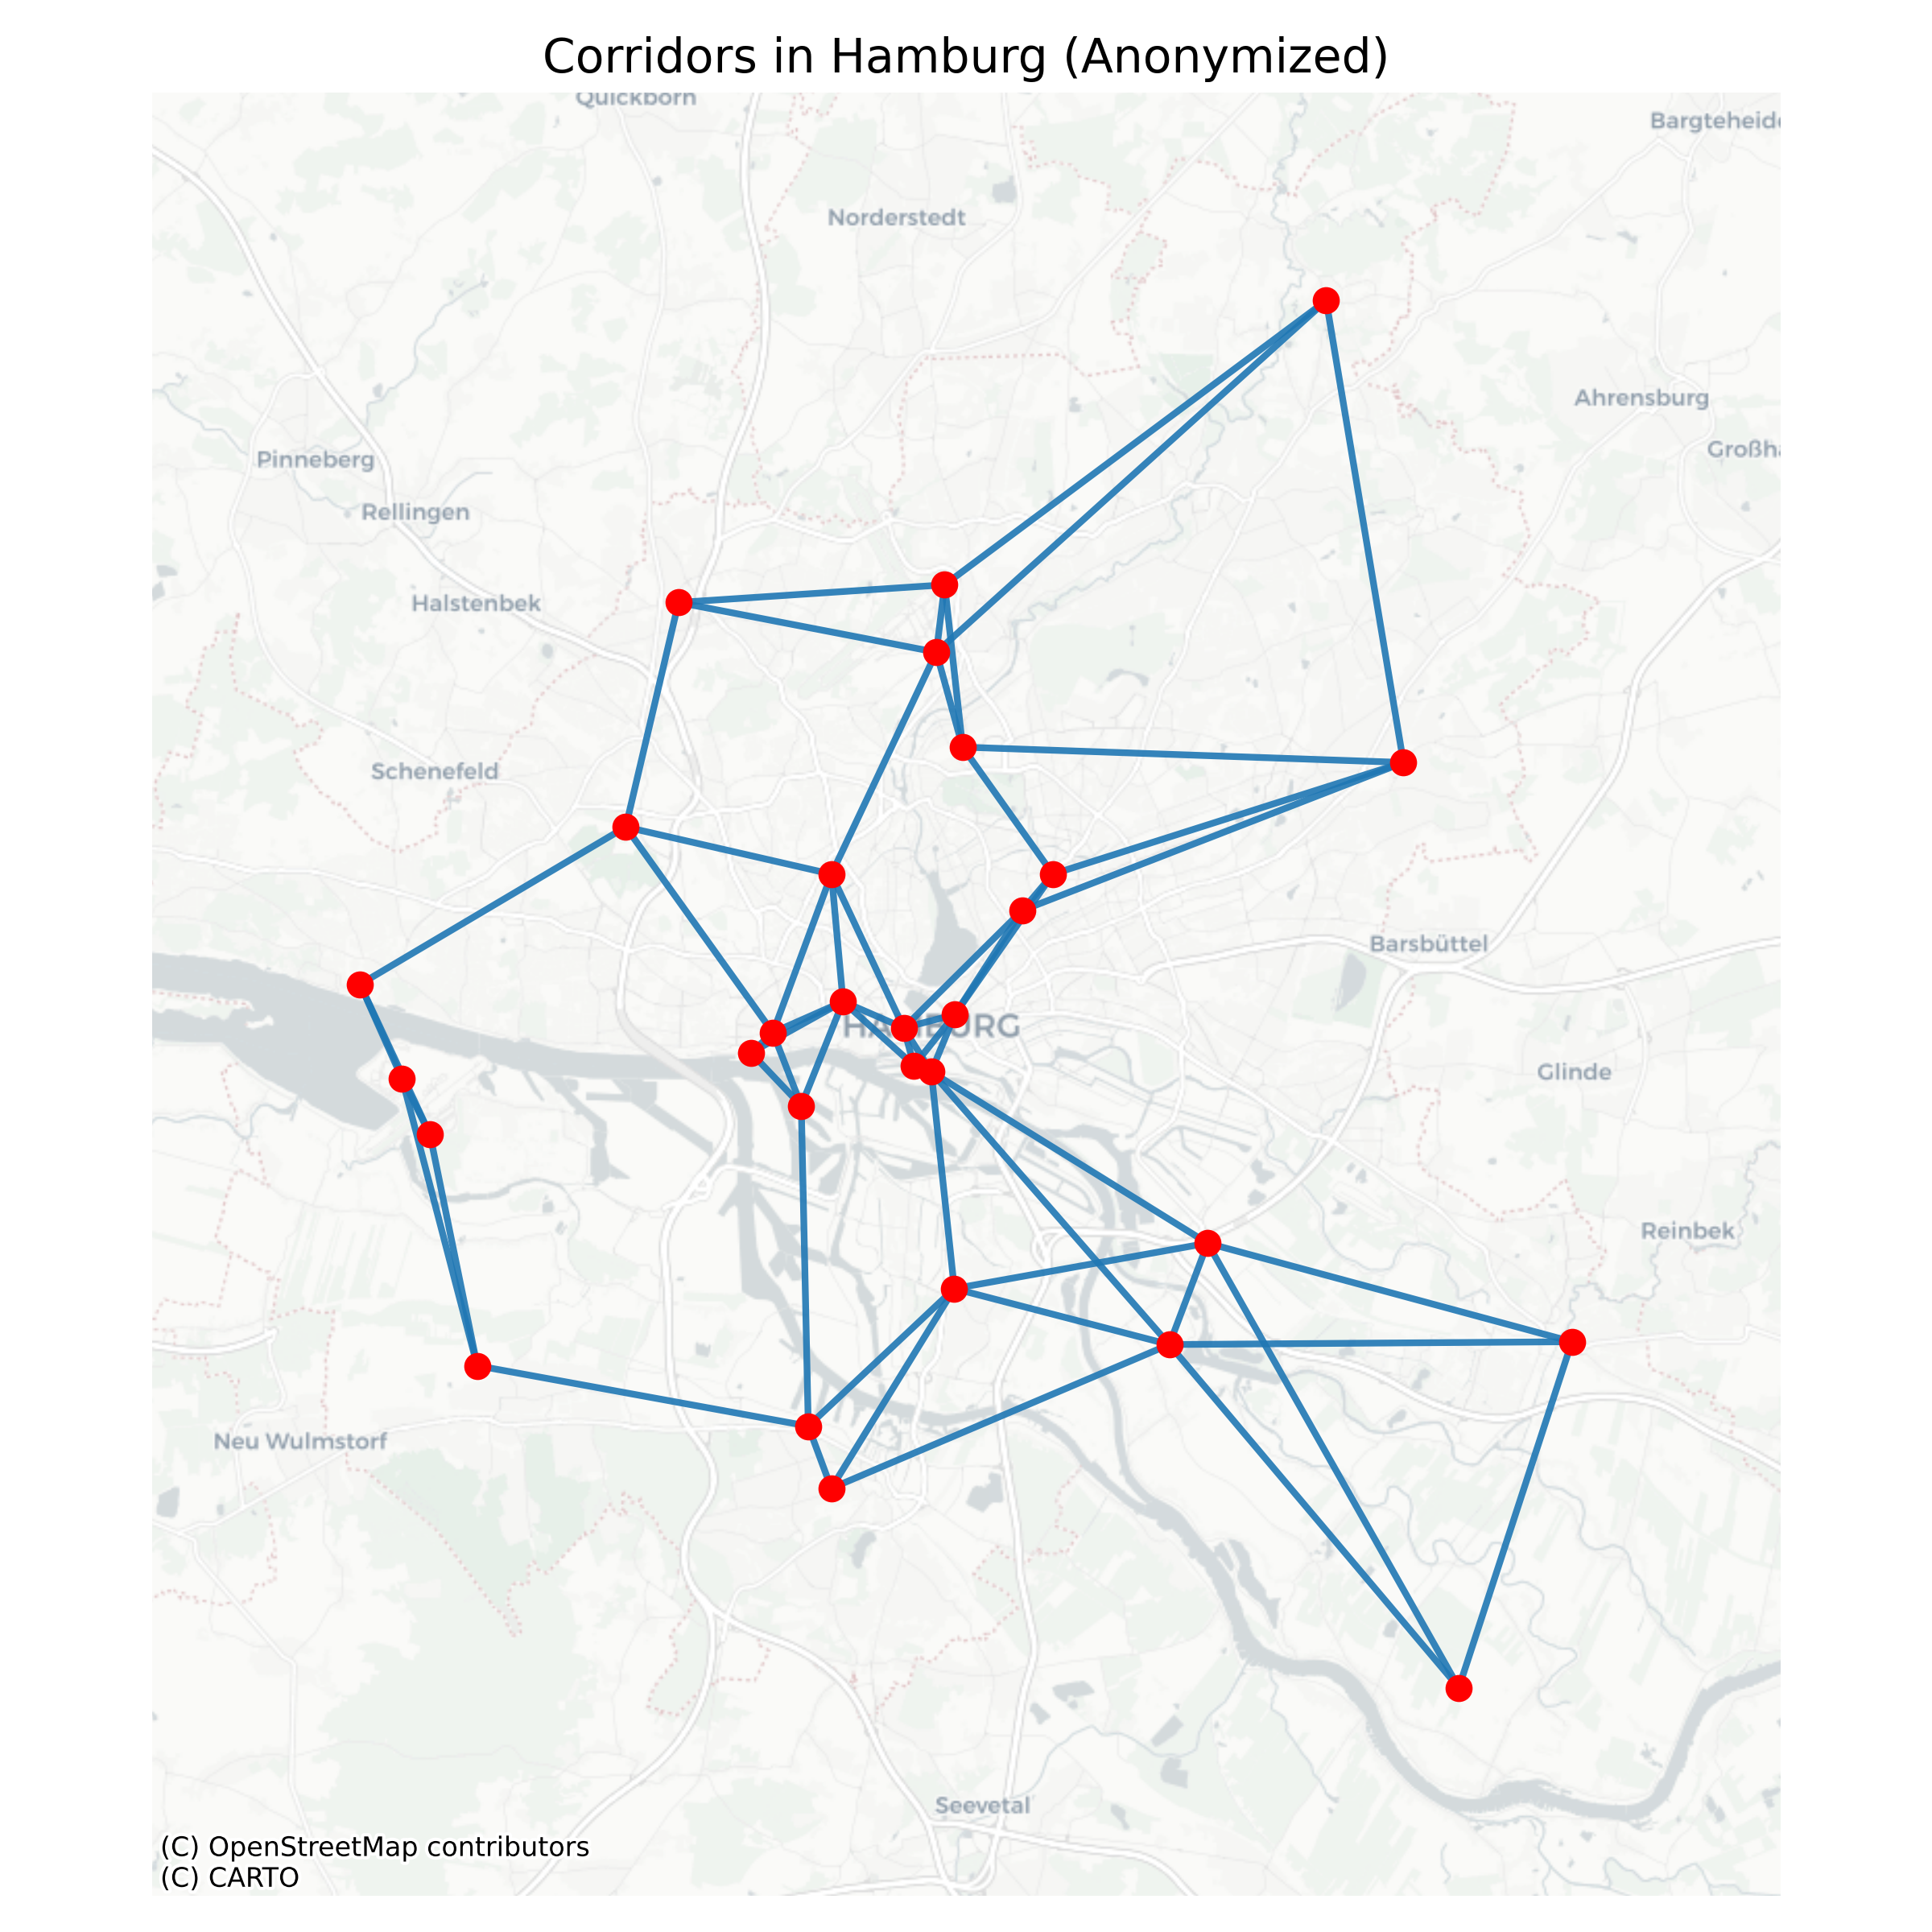
\includegraphics[width=\textwidth]{figures/corridors_hamburg.png}
    \caption{Constructed corridor network (static map view).}
    \label{fig:corridors_static}
  \end{subfigure}
  \hfill
  \begin{subfigure}{0.48\textwidth}
    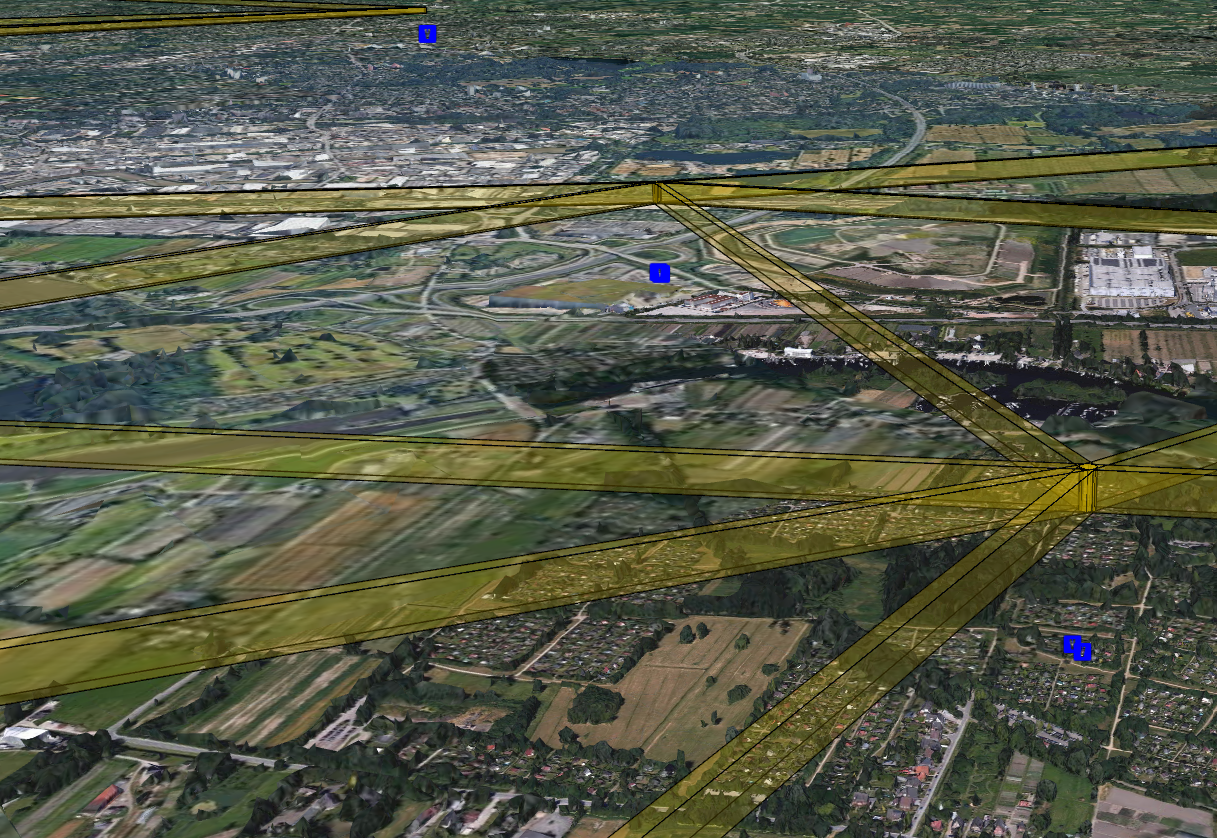
\includegraphics[width=\textwidth]{figures/corridors_hamburg_cesium.png}
    \caption{Cesium front-end view of the same corridor network (3D visualization).}
    \label{fig:corridors_cesium}
  \end{subfigure}
  \caption{Comparison of the corridor network in static map view (left) and interactive Cesium front-end (right).}
  \label{fig:corridors_comparison}
\end{figure}


\section{Graph Representation}
The resulting dataset is an \emph{undirected}, weighted graph in which nodes
correspond to vertiports and edges represent corridors. Edge weights are given
by geodesic distances between node coordinates. This graph serves as the basis
for all path planning experiments in this thesis; the global A* planner
(Sec.~\ref{sec:astar_global}) operates on this graph and uses the notation
$s$ (start), $n$ (current node), and $d$ (destination).
